\documentclass[12pt]{article}
\usepackage[a4paper, total={6in, 8in}]{geometry}
\usepackage{amsfonts}
\usepackage{amsmath,amssymb,trimclip,adjustbox}
\usepackage{breqn}
\usepackage{multirow}
\usepackage{geometry}
\usepackage{hyperref}
\usepackage{tabularray}
\usepackage{makecell}
\usepackage{flafter} 
\usepackage{polski}
\usepackage[utf8]{inputenc}

\geometry{top=2cm}

\setlength{\parindent}{0pt}
\setlength{\textheight}{720pt}
\setlength{\oddsidemargin}{0pt}
\setlength{\textwidth}{480pt}

\everymath{\displaystyle}


\author{Michał Puchyr}
\title{Sprawozdanie z ćw 17 \\
WYZNACZANIE WARTOŚCI PRZYSPIESZENIA ZIEMSKIEGO}

\begin{document}
\maketitle

\section{Cel ćwiczenia}

\begin{itemize}
    \item Wyznaczenie wartości przyspieszenia ziemskiego za pomocą wahadła matematycznego.
    \item Wyznaczenie wartości przyspieszenia ziemskiego za pomocą wahadła fizycznego.
\end{itemize}

\section{Opis ćwiczenia - wstęp teoretyczny}

Pomiary, które zostały wykonane miały na celu wyznaczenie \textbf{przyśpieszenia ziemskiego} w miejscu
gdzie był wykonywany eksperyment (Wrocław - $51^{\circ}06'27.7" N, 17^{\circ}03'40.6" E$). \\

\textbf{Przyspieszenie ziemskie} -- przyspieszenie grawitacyjne ciał swobodnie spadających na Ziemię, bez oporów ruchu.

Wartość przyspieszenia ziemskiego zależy od szerokości geograficznej oraz wysokości nad poziomem morza. 
Wraz z wysokością przyspieszenie maleje odwrotnie proporcjonalnie do kwadratu odległości do środka Ziemi 
i jest wynikiem zmniejszania się siły grawitacji zgodnie z prawem powszechnego ciążenia. 

Zmniejszanie się przyspieszenia ziemskiego wraz ze zmniejszaniem szerokości geograficznej 
jest spowodowane działaniem pozornej siły odśrodkowej, która powstaje na skutek ruchu obrotowego Ziemi. 

Ponieważ siła ta jest proporcjonalna do odległości od osi obrotu, stąd największą wartość osiąga na równiku. 
Ponieważ siła odśrodkowa ma tu zwrot przeciwny do siły grawitacji, 
przyspieszenie ziemskie na równiku osiąga najmniejszą wartość. 

Dodatkowe zmniejszenie przyspieszenia ziemskiego w okolicach równika spowodowane jest spłaszczeniem Ziemi 
(większą odległością od środka Ziemi).

Do obliczeń niewymagających wysokiej precyzji przyjmuje się tzw. przyśpieszenie ziemskie normalne tj.:
$$ g_n = 9,80665 \ \frac{m}{s^2} $$

Przyśpieszenie ziemskie we Wrocławiu wynosi około :
$$ g = 9,8115 \ \frac{m}{s^2} $$

\begin{center}
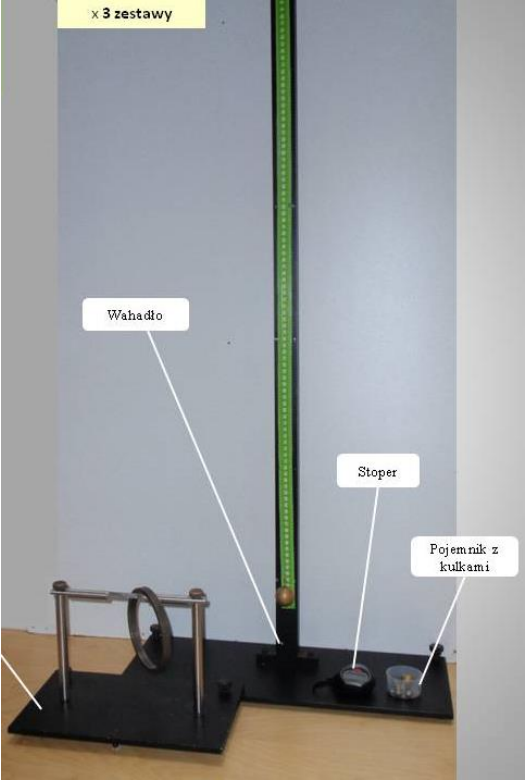
\includegraphics[scale=0.6]{schemat.png} \\
Stanowisko pomiarowe \\
\end{center}

Wykaz przyrządów : 
\begin{itemize}
    \item Wahadło matematyczne
    \item Metalowy pierścień
    \item Waga laboratoryjna
    \item Suwmiarka
    \item Stoper
    \item Przymiar
\end{itemize}

\section{Pomiary układów}

\begin{table}[!htbp]
    \centering
    \begin{adjustbox}{width=0.4\textwidth}
    \begin{tabular}{|c|c|}
    \hline
    \multicolumn{2}{|c|}{Przyjęte niepewności} \\
    \hline
    Niepewność & Wartość \\ \hline
    u(t)[s] & 0,0058 \\ \hline
    u(n) & 1 \\ \hline
    u(m)[kg] & 0,001 \\ \hline
    u(d)[m] & 0,001 \\ \hline
    \end{tabular}
\end{adjustbox}
\end{table}

\begin{table}[!htbp]
    \centering
    \begin{adjustbox}{width=1\textwidth}
    \begin{tabular}{|c|c|c|c|c|c|c|c|c|c|c|c|}
    \hline
    \multicolumn{10}{|c|}{Wyniki pomiarów i obliczenia dla wahadła matematycznego} \\
    \hline
    lp. & l$_i$[m] & t$_i$[s] & l$_{sr}$[m] & $\overline{t}$[s] & T$\left[ \frac{1}{s} \right]$ & u(T)$\left[\frac{1}{s}\right]$ & T$_{sr}\left[ \frac{1}{s} \right]$ & g$\left[ \frac{m}{s^2} \right]$ & $u_c(g) \left[ \frac{m}{s^2} \right] $
    \\[10pt] \hline
    1 & 0,390 & 125,15 & 0,391 & 125,01 & 1,26 & 0,013 & 1,25 & 9,699 & 0,247\\
    2 & 0,390 & 124,87 & ~ & ~ & 1,25          & 0,013 & ~     & 9,854 & 0,252\\
    3 & 0,391 & 124,98 & ~ & ~ & 1,25          & 0,013 & ~     & 9,880 & 0,253\\ \hline
    4 & 0,500 & 141,33 & 0,500 & 141,44 & 1,42 & 0,015 & 1,42  & 9,790 & 0,236\\
    5 & 0,501 & 141,46 & ~ & ~ & 1,42          & 0,015 & ~     & 9,809 & 0,237\\
    6 & 0,499 & 141,51 & ~ & ~ & 1,42          & 0,015 & ~     & 9,770 & 0,236\\ \hline
    7 & 0,613 & 156,48 & 0,614 & 156,47 & 1,57 & 0,016 & 1,57  & 9,818 & 0,221\\
    8 & 0,613 & 156,78 & ~ & ~ & 1,57          & 0,016 & ~     & 9,818 & 0,221\\
    9 & 0,614 & 156,13 & ~ & ~ & 1,57          & 0,016 & ~     & 9,834 & 0,221\\ \hline
    \multicolumn{8}{|r|}{$\overline{g} \left[ \frac{m}{s^2} \right]$} & \multicolumn{2}{|c|}{9,808} \\ \hline
    \multicolumn{8}{|r|}{$u(g) \left[ \frac{m}{s^2} \right]$} & \multicolumn{2}{|c|}{0,018} \\ \hline
    \end{tabular}
\end{adjustbox}
\end{table}

\begin{table}[!htbp]
    \centering
    \begin{adjustbox}{width=1\textwidth}
    \begin{tabular}{|c|c|c|c|c|c|c|c|c|c|c|c|c|}
    \hline
    \multicolumn{11}{|c|}{Wyniki pomiarów i obliczenia dla wahadła fizycznego} \\
    \hline
    lp. & m[kg] & d[m] & D[m] & I[kgm\textsuperscript{2}] & n & t$_i$[s] & T$\left[\frac{1}{s} \right]$  & u(T)$\left[\frac{1}{s} \right]$ & g$\left[\frac{m}{s^2}\right]$ & u$_c$(g)$\left[ \frac{m}{s^2} \right]$ 
    \\[10pt]
    \hline
    1 & \multirow{3}{*}{0,254} & \multirow{3}{*}{0,13} & \multirow{3}{*}{0,14} & \multirow{3}{*}{0,0023} & \multirow{3}{*}{100} & 73,74 & 0,738 & 0,008 & 10,098 & 0,221 \\
    \cline{7-11}
    2 &  & ~ & ~ & ~ & ~ & 73,71 & 0,738 & 0,008 & 10,098 & 0,221 \\
    \cline{7-11}
    3 &  & ~ & ~ & ~ & ~ & 73,54 & 0,736 & 0,008 & 10,153 & 0,223 \\ \hline
    \multicolumn{9}{|r|}{$\overline{g}\left[ \frac{m}{s^2} \right]$} & \multicolumn{2}{|c|}{10,117} \\ \hline
    \multicolumn{9}{|r|}{$u(g)\left[ \frac{m}{s^2} \right]$} & \multicolumn{2}{|c|}{0,222} \\ \hline
    \end{tabular}
\end{adjustbox}
\end{table}



\section{Przykładowe obliczenia}

\subsection{Obliczenia wspólne dla dwóch pomiarów}

Poniżej zostały zamieszczone obliczenia, które są wspólne dla obu pomiarów w celu wyeliminowania powtarzających się treści, jest to np.
obliczenie średniego czasu pomiarów, okresu wahnięć itd. \\

Obliczenie okresu wahnięć pomiaru :
$$ T = \frac{t_i}{n} = \frac{125,15}{100} = 1,2515 \approx 1,26 \left[ \frac{1}{s} \right] $$

Obliczenie średniej czasu pomiarów : 
$$ \overline{t} = \frac{\sum\limits_{i=1}^{n} t_i}{n} = \frac{375,01}{3} = 125,0033 \approx 125,01[s] $$

Obliczenie średniej długości okresu pomiarów :
$$ T_{sr} = \frac{\sum\limits_{i = 1}^{n} T_i}{n} = \frac{3,76}{3} = 1,25333 \approx 1,25\left[ \frac{1}{s} \right] $$

Obliczenie niepewności pomiaru okresu : 
$$ u(T) = \sqrt{ \left( \frac{\partial T}{\partial t} \right)^2 \cdot u^2(t) + \left( \frac{\partial T}{\partial n} \right)^2 \cdot u^2(n) }
= \sqrt{ \left( \frac{1}{n^2} \right)^2 \cdot u^2(t) + \left( \frac{-t}{n^2} \right)^2 \cdot u^2(n) } $$
$$ = \sqrt{ \left( \frac{1}{100^2} \right)^2 \cdot 0,0058^2 + \left( \frac{-125,15}{100^2} \right)^2 \cdot 1^2 } = 0,01251 \approx 0,013 \left[ \frac{1}{s} \right]$$

\subsection{Obliczenia dla pomiarów wahadła matematycznego}

Obliczenie niepewności pomiaru długości wahadła :
$$ u(l) = \frac{0,01}{\sqrt{3}} = 0,00578 \approx 0,0058[m] $$

Obliczenie przyśpieszenia ziemskiego : 
$$ g = 4\pi^2 \frac{l}{T^2} = 4\pi^2 \frac{0,390}{1,26^2} = 9,69802 \approx 9,699 \left[ \frac{m}{s^2} \right] $$

Obliczenie odchylenia standardowego pomiarów przyśpieszenia ziemskiego :
$$ u(g) = \sqrt{ \frac{\sum\limits_{i=1}^n (x_i - \overline{x})^2}{n(n-1)} } = \sqrt{ \frac{0,022}{72} } = 0,017411 \approx 0,018 \left[\frac{m}{s^2} \right] $$ 

Obliczenie średniej długości wahadła :
$$ l_{sr} = \frac{\sum\limits_{i=1}^{n} l_i}{n} = \frac{1,171}{3} = 0,39033 \approx 0,391[m]$$

Obliczenie niepewności całkowitej pomiaru przyśpieszenia ziemskiego :
$$ u(g) = \sqrt{ \left( \frac{\partial g}{\partial l} \right)^2 \cdot u^2(l) + \left( \frac{\partial g}{\partial T} \right)^2 \cdot u^2(T) }
= \sqrt{ \left( \frac{4 \pi^2}{T^2} \right)^2 \cdot u^2(l) + \left( \frac{-8 \pi^2 l}{T^3} \right)^3 \cdot u^2(T) } $$
$$ = \sqrt{ \left( \frac{4\pi^2}{1,26^2} \right)^2 \cdot 0,0058^2 + \left( \frac{-8\pi^2 \cdot 0,39}{1,26^3} \right)^2 \cdot 0,013^2 }
= 0,24667 \approx 0,247 \left[ \frac{m}{s^2} \right] $$


\subsection{Obliczenia dla pomiarów wahadła fizycznego}

Wzór na moment bezwładności :
$$ I = I_0 + m \frac{d^2}{4} $$

$$ I_0 = \frac{1}{8}m (d^2 + D^2) $$

gdzie
\begin{itemize}
    \item $I_0$ -- moment bezwładności pierścienia względem osi przechodzącej przez środek masy,
    \item $d$ -- średnica wewnętrzna, 
    \item $D$ -- średnica wewnętrzna pierścienia
\end{itemize}

Obliczenie moment bezwładności pierścienia względem osi przechodzącej przez środek masy : 
$$ I_0 = \frac{1}{8} \cdot 0,257 (0,13^2 + 0,14^2) = 0,00117 \approx 0,0012 [kg \cdot m^2] $$

Obliczenie momentu bezwładności pierścienia :
$$ I = 0,0012 + 0,0257 \cdot \frac{0,13^2}{4} = 0,002273 \approx 0,0023 [kg \cdot m^2] $$

Obliczenie przyśpieszenia ziemskiego :
$$ g = 8 \pi^2 \frac{I}{T^2 md} = 10,0978 \approx 10,098 \left[ \frac{m}{s^2} \right] $$ 

Obliczenie niepewności przyśpieszenia ziemskiego :
$$ u_c(g) = \sqrt{ \left( \frac{\partial g}{\partial T} \right)^2 \cdot u^2(T) + 
\left( \frac{\partial g}{\partial m} \right)^2 \cdot u^2(m) + \left( \frac{\partial g}{\partial d} \right)^2 \cdot u^2(d) } $$
$$ = \sqrt{ \left( -\frac{16\pi^2 I}{T^3 md} \right)^2 \cdot u^2(T) + \left( -\frac{8\pi^2 I}{T^2 m^2 d} \right)^2 \cdot u^2(m) + \left( -\frac{8\pi^2 I}{T^2 md^2} \right)^2 \cdot u^2(d) } $$
$$ = \sqrt{ \left( -\frac{16\pi^2 \cdot 0,0023}{0,738^3 \cdot 0,254 \cdot 0,13} \right)^2 \cdot 0,008^2 + }
$$ $$ \overline{\left( -\frac{8\pi^2 \cdot 0,0023}{0,738^2 \cdot 0,254^2 \cdot 0,13} \right)^2 \cdot 0,001^2 + 
\left( -\frac{8\pi^2 \cdot 0,0023}{0,738^2 \cdot 0,254 \cdot 0,13^2} \right)^2 \cdot 0,001^2 } $$
$$ = 0,22067 \approx 0,221 \left[\frac{m}{s^2}\right] $$

\section{Wnioski}

Przy pomocy pomiarów wahadła matematycznego i fizycznego zostały wyznaczone przybliżone wartości przyśpieszenia ziemskiego oddziałującego we Wrocławiu.
We wstępie teoretycznym przywołane zostało faktyczne przybliżenie przyśpieszenia ziemskiego we Wrocławiu 
$$ g = 9,8115 \ \frac{m}{s^2} $$.

Z pomiarów wahadła matematycznego średnie wyznaczone przyśpieszenie ziemskie wynosi około :
$$ g = 9,808 \pm 0,018 \ \frac{m}{s^2} $$

Z pomiarów wahadła fizycznego średnie wyznaczone przyśpieszenie fizyczne wynosi około :
$$ g = 10,117 \pm 0,222 \ \frac{m}{s^2} $$

Pomiary wykazały zbieżność ze znanym przyśpieszeniem ziemskim w miejscu wykonwywania eksperymentów. W przypadku wahadła 
fizycznego pomiar przyśpieszenia ziemskiego różni bardziej znacząco od faktycznego i zmierzonego przy użyciu wahadła matematycznego.

Na niewielką rozbieżność względem faktycznego przyspieszenia wpływają czynniki takie jak, krótki czas wahnięcia pierścienia,
niedokładność odmierzenia kąta wypuszczenia pierścienia oraz niewielka liczba wykonanych pomiarów w porównaniu do liczby pomiarów wahadła matematycznego. \\

\section{Bibliografia}
\begin{itemize}
    \item \url{https://pl.wikipedia.org/wiki/Przyspieszenie_ziemskie}
\end{itemize}

\end{document}